\section{Analysis and Asymptotic Notation}

\begin{frame}
  \frametitle{Analysing Algorithms}

  \begin{block}{Goal}
    \begin{itemize}
     \item Predict the resources that an algorithm requires
       \begin{itemize}
         \item computational time \pause (most often)
         \item memory, communication bandwidth, computer hardware\pause
       \end{itemize}
     \item \ldots often ignoring tedious details
     \end{itemize}  
  \end{block}
\end{frame}

\begin{frame}
    \begin{block}{General idea}
      \begin{itemize}
       \item The computational time taken to run an algorithm (such as
       InsertionSort) depends on the size of the input (e.g., the size $n$
       of the array).\pause In the case of InsertionSort,
       it also depends on how nearly sorted the elements of the array already are.

       \item We might describe the running time as a function of the input size.
         The input size depends of the problem (the size of an array, the number of
          vertices and edges of a graph, and so on). 

    \end{itemize}
  \end{block}  

\end{frame}

\begin{frame}
  The computational running time of an algorithm on a particular input is the
  number of primitive operations or steps executed. \pause We
  assume that a constant amount of time is necessary to
  execute each line of a pseudocode. \pause Due to repetitions, the
  same statement might be executed many times. 

  \begin{block}{Example: InsertionSort}
    \begin{itemize}
    \item For a given array $A[1 \ldots n]$, our goal is to
      {\bf estimate} the running time of the algorithm (in terms of
      a function $T(n)$). 
    \end{itemize}
  \end{block}
\end{frame}


\begin{frame}{InserctionSort}

  \begin{block}{Pseudocode for Insertion Sort}
\begin{scriptsize}
    \begin{algorithmic}
    \Procedure{InsertionSort}{A}
       \For{$j = 2, \dots, A.length$}            
         \State $key \gets A[j]$                 
         \State $i \gets j-1$                    
         \While{$i > 0\ and\ A[i] > key$}        
            \State $A[i+1] \gets A[i]$           
            \State $i \gets i - 1$               
         \EndWhile
         \State $A[i+1] = key$                   
       \EndFor
    \EndProcedure
    \end{algorithmic}
  \end{scriptsize}  
  \end{block}
\end{frame} 

\begin{frame}
  The computational running time of an algorithm on a particular input is the
  number of primitive operations or steps executed. \pause We
  assume that a constant amount of time is necessary to
  execute each line of a pseudocode. \pause Due to repetitions, the
  same statement might be executed many times. 

  \begin{block}{Example: InsertionSort}
    \begin{itemize}
    \item For a given array $A[1..n]$, our goal is to
      {\bf estimate} the running time of the algorithm ($T(n)$).

    \item But note that the cost of the {\bf while loop} is
      a function of the variable $j$ (that is, we can
      model the number of times the {\bf while loop condition} is executed
      as $T(j)$).
    \end{itemize}
  \end{block}
\end{frame}



\begin{frame}{InserctionSort}

  \begin{block}{Pseudocode for Insertion Sort}
\begin{scriptsize}
    \begin{algorithmic}
    \Procedure{InsertionSort}{A}
       \For{$j = 2, \dots, A.length$}             \Comment{Cost $c_1$ runs $n$ times}
         \State $key \gets A[j]$                  \Comment{Cost $c_2$ runs $n-1$ times}
         \State $i \gets j-1$                     \Comment{Cost $c_3$ runs $n-1$ times}
         \While{$i > 0\ and\ A[i] > key$}         \Comment{Cost $c_4$ runs $\sum_{j=2}^{n}t_j$ times}
            \State $A[i+1] \gets A[i]$            \Comment{Cost $c_5$ runs $\sum_{j=2}^{n}(t_j - 1)$ times}
            \State $i \gets i - 1$                \Comment{Cost $c_6$ runs $\sum_{j=2}^{n}(t_j - 1)$ times}
         \EndWhile
         \State $A[i+1] = key$                    \Comment{Cost $c_7$ runs $n-1$ times}
       \EndFor
    \EndProcedure
    \end{algorithmic}
  \end{scriptsize}  
  \end{block}
\end{frame} 

\begin{frame}
  \begin{multline*}
    T(n)  =  c_1n + c_2(n-1) + c_3(n-1) + c_4\sum_{j=2}^{n}t_j + c_5\sum_{j=2}^{n}(t_j - 1) \\ + c_6\sum_{j=2}^{n}(t_j - 1) + c_7(n-1)
  \end{multline*}
\pause
  \begin{itemize}
   \item Best case: array is already sorted
   \item Worst case: the array is in reverse sorted order 
  \end{itemize}
  
\end{frame}

\begin{frame}{Best case: $T(j) = 1$}
  \begin{multline*}
    T(n)  =  c_1n + c_2(n-1) + c_3(n-1) + c_4(n-1) + c_7(n-1) = \\
             (c_1 + c_2 + c_3 + c_4 + c_7)n - (c2 + c3 + c4 + c7) 
  \end{multline*}

  \pause
  
  \begin{itemize}
    \item $T(n)$ is a linear function of $n$.
  \end{itemize}

\end{frame}

\begin{frame}{Worst Case: $T(j) = j$, for $j=2, 3, \ldots, n$}

  \begin{block}{Note that}
    \begin{itemize}
      \item $\sum_{j=2}^{n}j = \frac{n(n+1)}{2}-1$
      \item $\sum_{j=2}^{n}(j-1) = \frac{n(n-1)}{2}$
    \end{itemize}
  \end{block}

\end{frame}

\begin{frame}

    \begin{multline*}
    T(n) = c_1n + c_2(n-1) + c_3(n-1) + c_4(\frac{n(n+1)}{2}-1) + c_5(\frac{n(n-1)}{2}) \\ + c_6(\frac{n(n-1)}{2}) + c_7(n-1)
    \end{multline*}

\end{frame}

\begin{frame}

    \begin{multline*}
      T(n) =   (\frac{c_4}{2} + \frac{c_5}{2} + \frac{c_6}{2})n^2 \\
              + (c_1 + c_2 + c_3 + \frac{c_4}{2} - \frac{c_5}{2} - \frac{c_6}{2} + c_7)n \\
              - (c_2 + c_3 + c_4 + c_7) 
    \end{multline*} \pause

    \pause
  
    \begin{itemize}
     \item $T(n)$ is a quadratic function of $n$ for the worst case. \pause
      We are often interested in finding only the {\bf worst-case running time}.
    \end{itemize}
\end{frame}

\begin{frame}

  \begin{itemize}
    \item More precisely, when we analyse an algorithm, we
      are more interested in the {\bf order of growth} of the (worst-case)
      running time of an algorithm. \pause For a function $an^2 + bn +c$, we
       consider only the leading term ($n^2$) ignoring all constants, since the lower-order
         terms and constants are insignificant for large values of $n$.
  \end{itemize}

  \pause
  
  \begin{block}{In summary}
    \begin{itemize}
    \item We say that InsertionSort has a worst-case running time of $\Theta(n^2)$\pause. For large
      enough inputs, a $\Theta(n^2)$ algorithm takes less time to execute than an algorithm whose
      worst case running time is $\Theta(n^3)$. \pause  
    \end{itemize}
  \end{block}
\end{frame}

\begin{frame}
  \begin{quote}
    ``For large enough inputs, the multiplicative constants and the lower-order terms
    of an exact running time are dominated by the effects of the input size itself.'' 
  \end{quote}
  \flushright{(Introduction to Algorithms, Cormen et al.)}

\end{frame}

\begin{frame}
  \begin{itemize}
  \item Asymptotic efficiency of algorithms: aims to understand
    how the running time of an algorithm increases with the size
    of the input in the limit. 
  \end{itemize}
\end{frame}

\begin{frame}{Asymptotic Notation}

  \centering{
    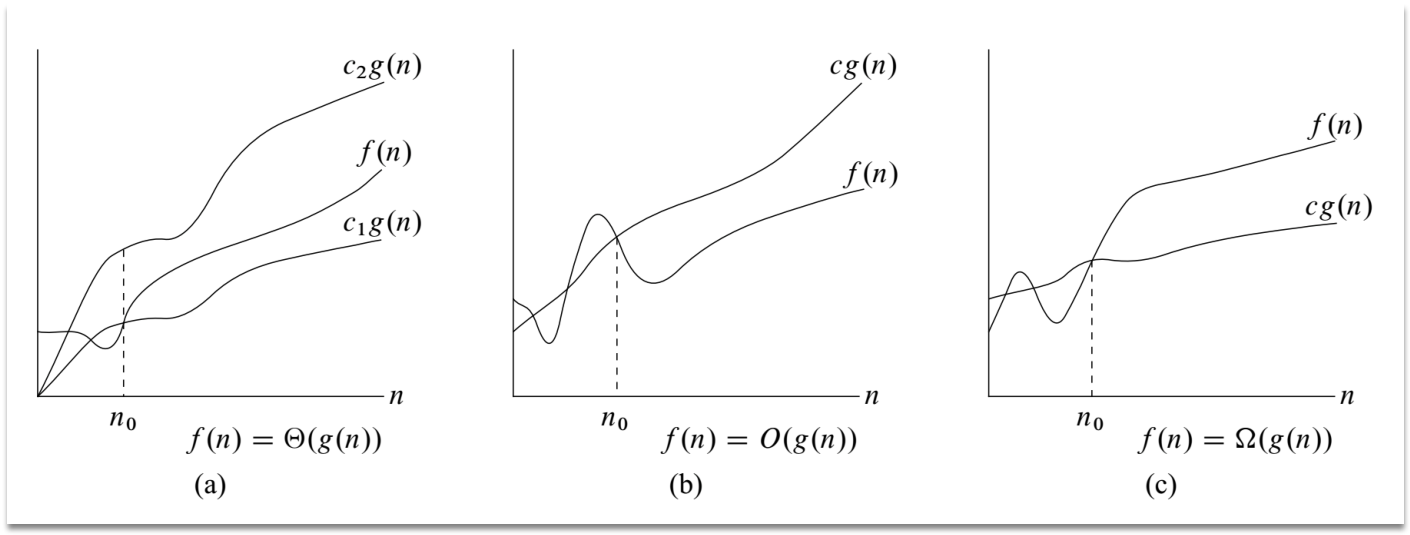
\includegraphics[scale=0.4]{images/asymptotic-notation.pdf}
  }
  \flushright{\itab}
  
\end{frame}

\begin{frame}{$\Theta$-notation}

  \begin{block}{Definition}
    \begin{itemize}
    \item For a given function $g(n)$, we define
      $\Theta(g(n))$ the set of functions:
    \end{itemize}
    
    \begin{small}
      \begin{multline*}
        \Theta(g(n)) = \{ f(n):\ there\ exist\ positive\ constants\ c_1,\ c_2,\ and\ n_0\ \\ such\ that\ 
                       0 \leq c_1g(n) \leq f(n) \leq c_2g(n)\ for\ all\ n \geq n0\}
      \end{multline*}
    \end{small}
  \end{block}

\end{frame}

\begin{frame}
  Example: $\frac{1}{2}n^2 - 3n \in \Theta(n^2)$ \pause

  \begin{itemize}
  \item We must determine positive constants $c_1$, $c_2$, and $n_0$,
    such that $c_1n^2 \leq \frac{1}{2}n^2 -3n \leq c2n^2$, for all $n \geq n_0$. \pause
  \item Possible solution for $n \geq 7$: \pause $c_1 \leq 1/14$ and $c_2 >= 1/2$.   
  \end{itemize} 
\end{frame}


\begin{frame}{$\mathcal{O}$-notation (asymptotic upper bound)}

  \begin{block}{Definition}
    \begin{itemize}
    \item For a given function $g(n)$, we define
      $\mathcal{O}(g(n))$ the set of functions:
    \end{itemize}
    
    \begin{small}
      \begin{multline*}
        \mathcal{O}(g(n)) = \{ f(n):\ there\ exist\ positive\ constants\ c,\ and\ n_0\ \\ such\ that\ 
                       0 \leq f(n) \leq cg(n)\ for\ all\ n \geq n0\}
      \end{multline*}
    \end{small}

    \begin{itemize}
      \item Note that $f(n) \in \Theta(g(n))$ implies $f(n) in \mathcal{O}(g(n))$  
    \end{itemize}
  \end{block}

\end{frame}

\begin{frame}{$\Omega$-notation (asymptotic lower bound)}

  \begin{block}{Definition}
    \begin{itemize}
    \item For a given function $g(n)$, we define
      $\Omega(g(n))$ the set of functions:
    \end{itemize}
    
    \begin{small}
      \begin{multline*}
        \Omega(g(n)) = \{ f(n):\ there\ exist\ positive\ constants\ c,\ and\ n_0\ \\ such\ that\ 
                       0 \leq c(g(n) \leq f(n)\ for\ all\ n \geq n0\}
      \end{multline*}
    \end{small}
  \end{block}

\end{frame}

\begin{frame}{$o$-notation (upper bound not asymptotically tight)}

  \begin{block}{Definition}
    \begin{itemize}
    \item For a given function $g(n)$, we define
      $\mathcal{o}(g(n))$ the set of functions:
    \end{itemize}
    
    \begin{small}
      \begin{multline*}
        o(g(n)) = \{ f(n):\ for\ any\ c > 0, there\ exists\ a\ positive\ constant\ n_0 > 0\ \\ such\ that\ 
                       0 \leq f(n) < cg(n) \ for\ all\ n \geq n0\}
      \end{multline*}
    \end{small}
  \end{block}

\end{frame}

\begin{frame}{$\omega$-notation (lower bound not asymptotically tight)}

  \begin{block}{Definition}
    \begin{itemize}
    \item For a given function $g(n)$, we define
      $\omega(g(n))$ the set of functions:
    \end{itemize}
    
    \begin{small}
      \begin{multline*}
        \omega(g(n)) = \{ f(n):\ for any c > 0, there\ exists\ a positive\ constant\ n_0 > 0\ \\ such\ that\ 
                       0 \leq cg(n) < f(n) \ for\ all\ n \geq n0\}
      \end{multline*}
    \end{small}
  \end{block}

\end{frame}


\begin{frame}{Running time of divide-and-conquer algorithms}

  \begin{itemize}
   \item Often involves a {\bf recurrence relation}. \pause
     The overall running time on a problem of size $n$ is described
     in terms of the running time on smaller inputs.

     \begin{itemize}
       \item Base case: when the input is small enough ($n \leq c$),
         the straightforward solution takes constant time ($T(n) = \Theta(1)$). \pause
         
       \item Recursive case: We split the problem into $a$ subproblems,
         each one having $\frac{1}{b}$ the size of the original input \pause(for MergeSort,
         $a = b = 2$). \pause Assuming we take $D(n)$ time to divide the problem into
         the subproblems and $C(n)$ to combine the solutions to the subproblems,
         we can derive a general solution for the running time of divide-and-conquer
         algorithms.
     \end{itemize}
  \end{itemize}
\end{frame}

\begin{frame}

  \begin{block}{General solution}
  \[ 
   T(n)= \left\{
   \begin{array}{ll}
     \Theta(1) & n \leq c, \\
     aT(n/b) + D(n) + C(n) & otherwise. \\
   \end{array} 
   \right. 
   \]
  \end{block}      

  \begin{itemize}
  \item There are three approaches for solving
    recurrence relations: the recursion-tree method,
    the substitution method, and the master method. 
  \end{itemize}
\end{frame}


\begin{frame}{Running time of MergeSort}

  Lets assume the input size is a power of 2 (1, 2, 4, 8, 16, 32, \ldots). pause
  Each divide step takes two subsequences of size $n/2$. \pause When we
  have $n > 1$ elements, we split the running time as follows:

  \begin{description}
   \item [Divide:] The divide step just computes the middle of the subarray (constant time).
     Therefore, $D(n) = \Theta(1)$.
   \item [Conquer:] The algorithm recursively solves two subproblems, each of size n/2.
     This contributes with $2T(n/2)$ to the running time.
     
   \item [Combine:] The merge procedure on $n$ elements takes time $\Theta(n)$, therefore
     $C(n) = \Theta(n)$
  \end{description}
\end{frame}

\begin{frame} 
  \[ 
   T(n)= \left\{
   \begin{array}{ll}
     \Theta(1) & if\ n = 1, \\
     2T(n/2) + \Theta(n) & if\ n > 1. \\
   \end{array} 
   \right. 
   \]
  
\end{frame}



\begin{frame}

  \[ 
   T(n)= \left\{
   \begin{array}{ll}
     c & if\ n = 1, \\
     2T(n/2) + cn & if\ n > 1. \\
   \end{array} 
   \right. 
   \]
  
\end{frame}

\begin{frame}

  \centering{
    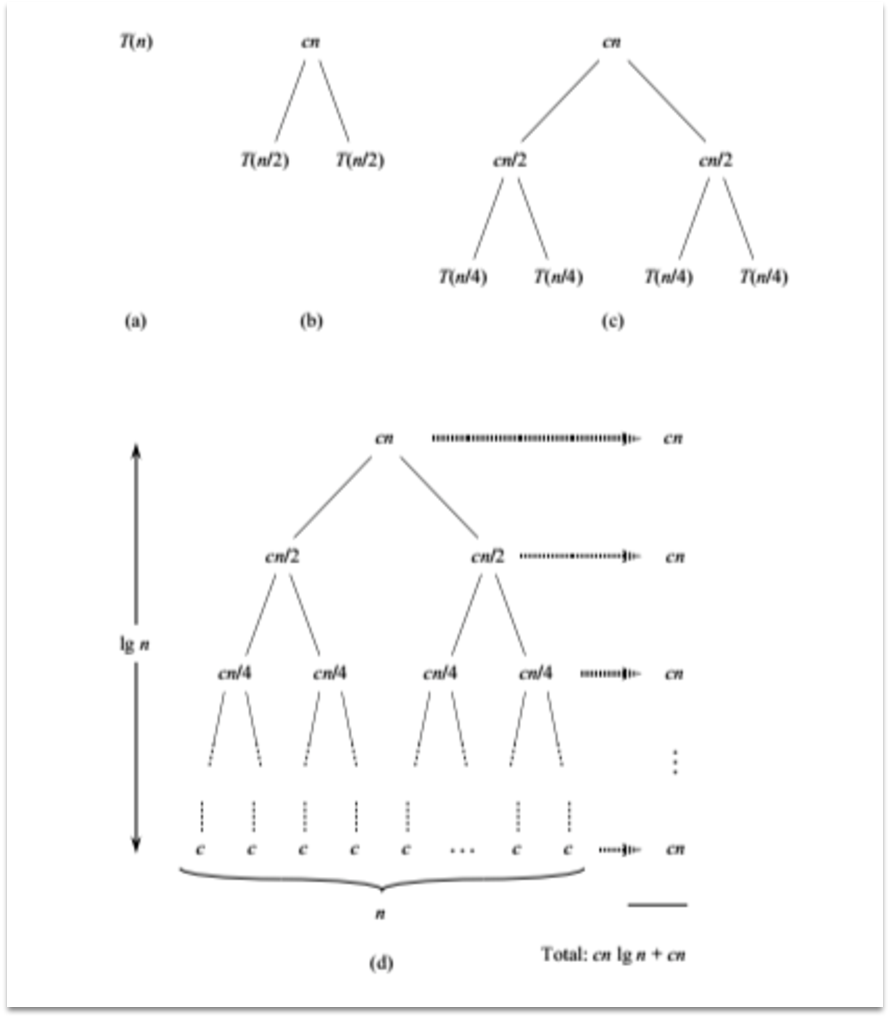
\includegraphics[scale=0.3]{images/recurrence-tree.pdf}
  }

  \flushright{\itab}
\end{frame}

\begin{frame}{The substitution method}
  \begin{block}{Two steps}
    \begin{itemize}
     \item Guess the form of the solution
     \item Proove that the solution works (using mathematical induction) 
    \end{itemize}
  \end{block}
\end{frame}

\begin{frame}{Example}

\begin{eqnarray*}
    T(n)  & = &  2T(\lfloor n/2 \rfloor) + n
\end{eqnarray*}  \pause

\begin{itemize}
\item Similar to the recurrence relation of the running time for MergeSort. \pause
  {\bf Guess}: the solution is $T(n) = \mathcal{O}(n log n)$. \pause So, we need to prove
  that $T(n) \leq c\ n\ log\ n$ for an appropriate choice of the const $c > 0$.
\end{itemize}
\end{frame}

\begin{frame}
\begin{itemize}
\item Lets assume this property holds for all positive $m < n$, in particular for
  $m = \lfloor n/2 \rfloor$. \pause This yields:

  \begin{eqnarray*}
    T(\lfloor n/2 \rfloor) & \leq & c \lfloor n/2 \rfloor log (\lfloor n/2 \rfloor)
  \end{eqnarray*}
      
\item  Substituting in the recurrence, we get:

  \begin{small}
\begin{eqnarray*}
  T(n) & \leq & 2  c \lfloor n/2 \rfloor log (\lfloor n/2 \rfloor) + n \\
       & \leq & c\ n\ log\ n/2 + n              \\
       & =    & c\ n\ log\ n - c\ n\ log\ 2 + n    \\
       & =    & c\ n\ log\ n - c\ n\ + n          \\
       & \leq & c\ n\ log\ n                    \\ 
 \end{eqnarray*}
  \end{small}
\end{itemize}
\end{frame}

\begin{frame}

\begin{itemize}
  \item It is also necessary to prove the base case (finding out a $n_0$ and $c$
    so that $T(n) \leq c\ n\ log\ n$). \pause T(1) does not hold for this example \pause, though for $n=2$ and
    $n=3$ it does.

  \item It is often necessary to elaborate the proof on some corner cases, by \emph{subtracting a lower-order term} or by
    \emph{changing variables}. The book covers these scenarios.     
\end{itemize}
\end{frame}


\begin{frame}{The (magic) master method}

  A ``cookbook'' for solving recurrences of the form:

  \begin{eqnarray*}
    T(n) & = & a\ T(n/b) + f(n)
  \end{eqnarray*}

   where $a \geq 1$, $b > 1$ and $f(n)$ is an asymptotivally positive function.

   \begin{block}{Three cases}
     \begin{scriptsize}
     \begin{itemize}
      \item if $f(n) = \mathcal{O}(n^{log_b a-\epsilon})$ for some constant $\epsilon > 0$\pause, then $T(n) = \Theta(n^{log_b a})$ \pause
      \item if $f(n) = \Theta(n^{log_b a})$\pause, then $T(n) = \Theta(n^{log_b a} log n)$\pause
      \item if $f(n) = \Omega(n^{log_b a + \epsilon})$ for some constant $\epsilon > 0$\pause, then $T(n) = \Theta(f(n))$ 
     \end{itemize}
     \end{scriptsize}
   \end{block}  
  
\end{frame}

\begin{frame}{Examples}

  \begin{itemize}
    \item $T(n) = 9T(n/3) + n$
    \item $T(n) = T(2n/3) + 1$
    \item $T(n) = 3T(n/4) + n\ log\ n$  
  \end{itemize}

\end{frame}
